\documentclass{beamer}

\title{Student wellbeing survey web application}
\author{Tarnjot Singh Virdee (24009864)}

\usetheme{Pittsburgh}

\begin{document}

\maketitle

\begin{frame}
\begin{columns}
    \column{.4\textwidth}
    15\% to 20\% of \emph{teens} suffer from some mental health issues

    \column{.6\textwidth}
    \includegraphics[height=1\textheight]{images/Mental-Health-1.jpg}

\end{columns}
\end{frame}

\begin{frame}
    \frametitle{Problem definition}
    \begin{itemize}
        \pause
        \item Have health experts create surveys 
        \pause
        \item Subscribed students can respond to them 
    \end{itemize}  
\end{frame}  

\begin{frame}
    \frametitle{Objectives}
    \begin{itemize}
        \pause
        \item Server side application 
        \begin{itemize}
            \item Manage databases
            \item Provide an API for client
        \end{itemize}

        \pause
        \vspace{.2cm}
        \item Client side application 
        \begin{itemize}
            \item Consumes the API
            \item Provide the necessary functionality
            \item Fast, simple to use
            \item Reusable code for future mobile app
        \end{itemize}

        \pause
        \vspace{.2cm}
        \item Allow for future scalability
    \end{itemize}    

\end{frame}

\begin{frame}
    \frametitle{High level architecture}
    \begin{columns}
        \column{.5\textwidth}
        \includegraphics[height=.75\textheight]{images/simple_solution_architecture.png}

        \column{.5\textwidth} 
        \begin{itemize}
            \pause
            \item Server running a Java SpringBoot application
            \begin{itemize}
                \item Provides a collection of REST API endpoints
            \end{itemize}
            
            \pause
            \vspace{.2cm}
            \item REACTjs front end client
            \begin{itemize}
                \item Uses the API to provide the necessary functionality
            \end{itemize}

            \pause
            \vspace{.2cm}
            \item Serves user requests
        \end{itemize}
    \end{columns}    
\end{frame}

\begin{frame}
    \frametitle{Security}
    \begin{columns}
        \column{.6\textwidth}
        \begin{itemize}
            \pause
            \item Oauth2 based authentication
            \begin{itemize}
                \item Secure resources exposed by API
                \item Issue tokens to client
            \end{itemize}

            \pause
            \vspace{.2cm}
            \item Json Web Tokens
            \begin{itemize}
                \item No need to manage sessions
                \item Increases scalability
            \end{itemize}

            \pause
            \vspace{.2cm}
            \item Bcrypt password encryption
            \begin{itemize}
                \item 10 rounds of encryption
            \end{itemize}
        \end{itemize}

        \pause
        \column{.5\textwidth}
        \includegraphics[height=.7\textheight]{images/simple_auth_flow.png}
    \end{columns}
    

\end{frame}

\begin{frame}
    \frametitle{Technologies overview}

    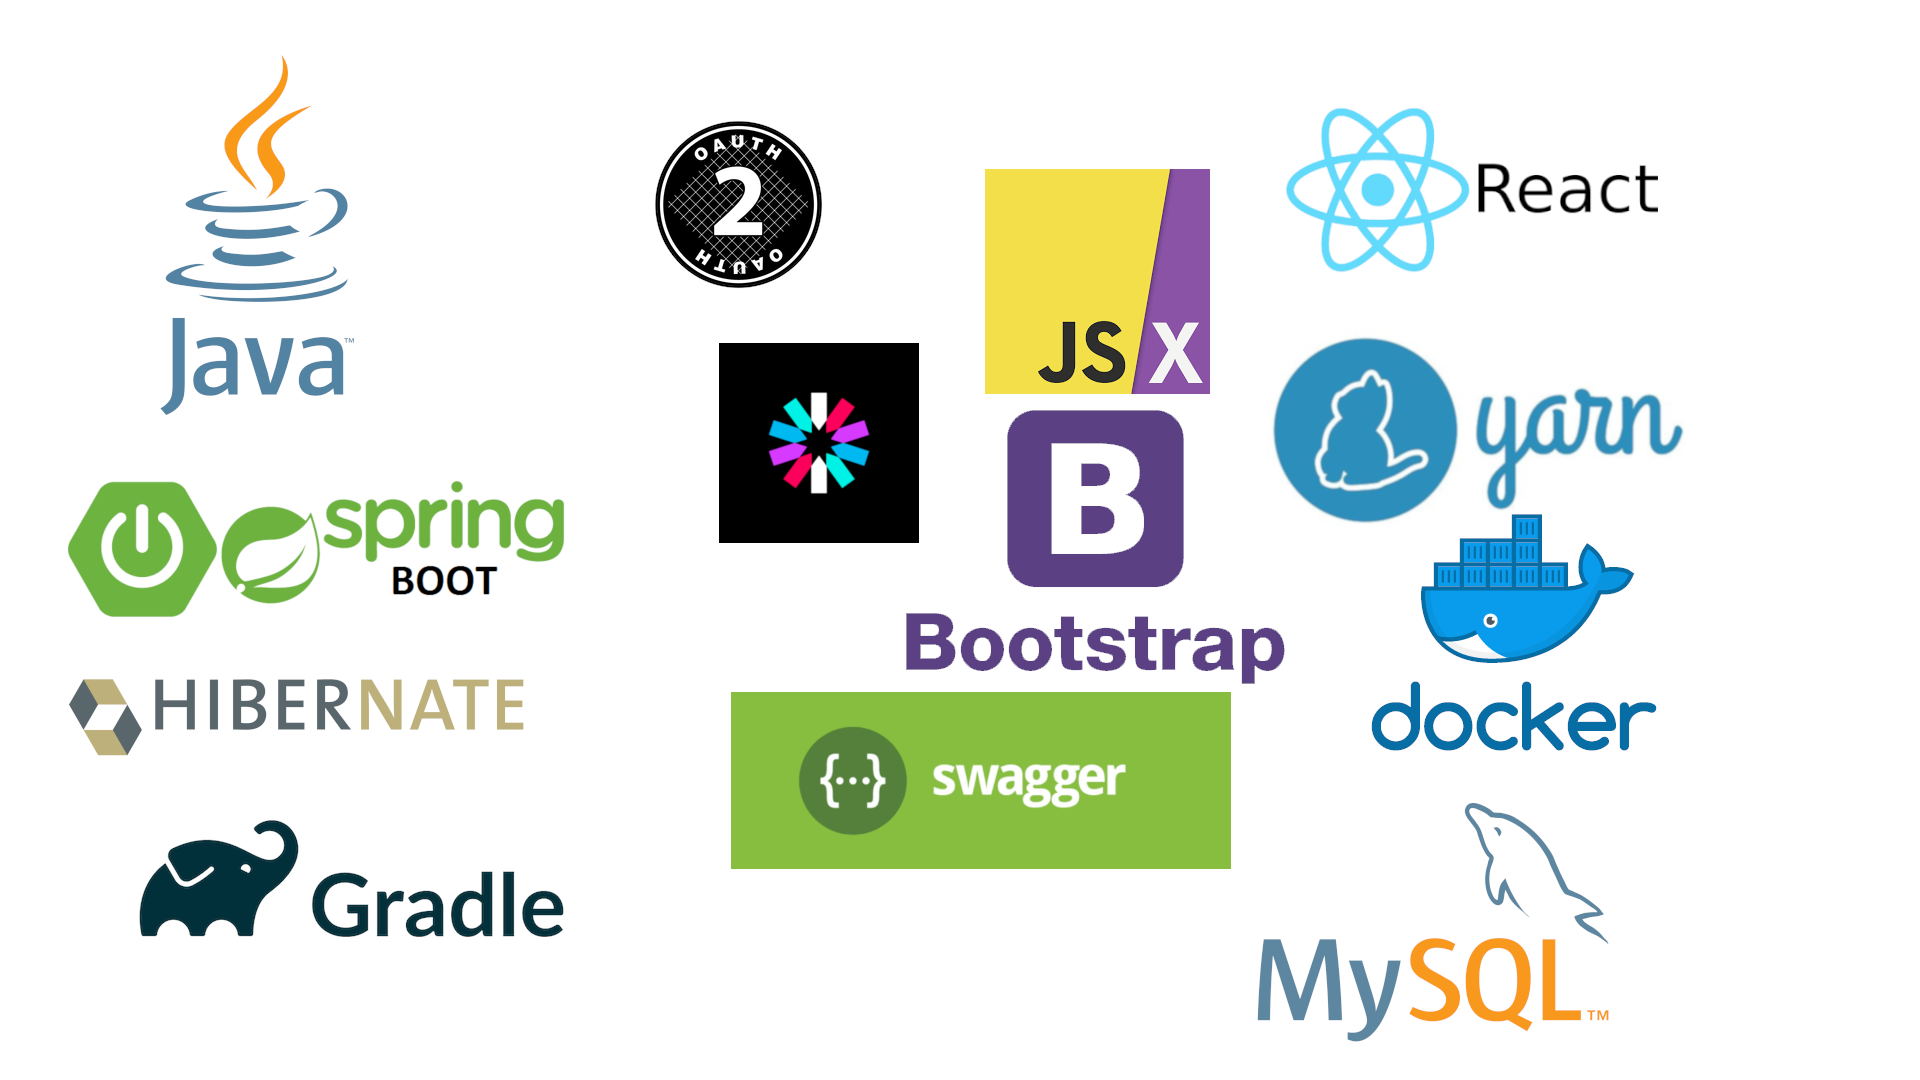
\includegraphics[width=1.1\textwidth]{images/logo_splash.png}

\end{frame}
\end{document}